\documentclass[12pt]{article}
\usepackage[utf8]{inputenc}
\usepackage[T1]{fontenc}
\usepackage{amsmath}
\usepackage{graphicx}
\usepackage{booktabs}
\usepackage{natbib}
\usepackage{url}
\usepackage{geometry}
\usepackage{setspace}
\usepackage{caption}
\usepackage{subcaption}

\geometry{margin=1in}
\doublespacing

\title{Testing the Grammatical Status of Reciprocals: \\
A Quantitative Feature-Based Analysis}

\author{[Author Name] \\
[Institution] \\
[Email]}

\date{\today}

\begin{document}

\maketitle

\begin{abstract}
This study tests the hypothesis that English reciprocals \textit{each other} and \textit{one another} are better classified as fused determinatives rather than pronouns, as traditionally assumed. Using a comprehensive linguistic feature matrix (139 items × 157 features), we applied multiple convergent analytical methods following rigorous statistical practices. Our analysis included permutation testing, model comparison, standard visualization techniques (Multiple Correspondence Analysis and Principal Coordinates Analysis), and Bayesian inference with informative priors. While most methods favored the traditional pronoun classification, focused distance analysis revealed closer similarity to fused determinatives, highlighting significant methodological sensitivity. The quantitative evidence suggests reciprocals occupy a genuinely intermediate grammatical position, though some apparent complexity may reflect analytical limitations rather than purely linguistic phenomena. These findings demonstrate both the potential and the challenges of quantitative approaches to contested grammatical classifications.
\end{abstract}

\section{Introduction}

The grammatical classification of English reciprocals \textit{each other} and \textit{one another} has been a subject of ongoing theoretical interest in linguistic research. While traditional analyses following major reference grammars such as \citet{huddleston2002cambridge} classify these forms as pronouns, recent theoretical work has proposed alternative classifications.

One particularly interesting proposal suggests that reciprocals might be better analyzed as fused determinatives—complex grammatical units that combine determinative and nominal functions \citep{payne2007fusion}. This classification would group reciprocals with items like \textit{someone}, \textit{anyone}, \textit{everything}, and \textit{somebody}, which exhibit similar morphological complexity and semantic-syntactic properties.

The fusion-of-functions framework \citep{payne2007fusion} provides theoretical motivation for this reclassification. Under this approach, grammatical categories are not discrete but can represent combinations of traditional functions. Reciprocals, with their complex morpho-syntactic properties and anaphoric behavior, could plausibly be analyzed as fused determinative-nominal units rather than simple pronouns.

However, testing such theoretical proposals requires empirical validation using comprehensive linguistic data. This study addresses this gap by applying quantitative methods to a large-scale feature matrix, testing whether reciprocals pattern more closely with fused determinatives or with traditional pronouns across multiple dimensions of linguistic analysis.

\subsection{Research Questions}

This study addresses the following specific research questions:

\begin{enumerate}
\item Do English reciprocals \textit{each other} and \textit{one another} show greater similarity to fused determinatives than to pronouns when measured across comprehensive linguistic features?
\item How robust is any observed pattern across different analytical methods and statistical approaches?
\item What theoretical implications follow from quantitative feature-based evidence regarding reciprocal classification?
\end{enumerate}

\section{Methodology}

\subsection{Data}

Our analysis employed a comprehensive linguistic feature matrix containing 139 linguistic items described across 157 binary features. The features encompass morphological, semantic, and syntactic properties representing diverse dimensions of grammatical behavior.

The dataset includes:
\begin{itemize}
\item \textbf{Reciprocals}: \textit{each other}, \textit{one another} (2 items)
\item \textbf{Fused determinatives}: \textit{someone}, \textit{anyone}, \textit{anything}, \textit{everything}, \textit{somebody}, \textit{anybody} (6 items)
\item \textbf{Pronouns}: 63 items including personal, demonstrative, and other pronominal forms
\item \textbf{Other categories}: Various determinatives, nouns, and other grammatical categories
\end{itemize}

\subsection{Analytical Approach}

Following best practices in quantitative linguistics and statistical methodology \citep{gelman2013bayesian}, we employed a multi-method approach with pre-registered hypotheses to avoid researcher degrees of freedom and ``forking paths'' in data analysis.

\subsubsection{Pre-registration}

Prior to analysis, we established:
\begin{itemize}
\item \textbf{Primary hypothesis}: Reciprocals should show greater similarity to fused determinatives than to pronouns if the reclassification proposal is correct
\item \textbf{Falsification criteria}: Failure to find significant clustering with fused determinatives would count as evidence against the hypothesis
\item \textbf{Prior expectations}: Strong prior (85\%) favoring traditional pronoun classification based on scholarly consensus
\end{itemize}

\subsubsection{Statistical Methods}

We applied four complementary analytical approaches:

\paragraph{1. Permutation Testing}
We tested whether reciprocals show preferential clustering with fused determinatives using permutation tests. This approach compares observed clustering patterns against null distributions generated by randomly reassigning category labels, providing robust significance testing without distributional assumptions.

\paragraph{2. Model Comparison}
We compared logistic regression models predicting grammatical category membership, testing whether models treating reciprocals as determinatives fit the data better than models treating them as pronouns.

\paragraph{3. Visualization and Ordination}
Following standard practices in computational linguistics, we employed:
\begin{itemize}
\item \textbf{Multiple Correspondence Analysis (MCA)}: The standard approach for categorical linguistic features
\item \textbf{Principal Coordinates Analysis (PCoA)}: Distance-based ordination using Jaccard distances, appropriate for binary sparse features
\end{itemize}

\paragraph{4. Bayesian Analysis}
We implemented Bayesian inference incorporating strong informative priors based on scholarly consensus, allowing principled integration of theoretical knowledge with empirical evidence.

\section{Results}

\subsection{Primary Hypothesis Test}

The permutation test found no significant evidence for preferential clustering of reciprocals with fused determinatives. Of the two reciprocals examined, only one showed closer proximity to fused determinatives than to pronouns (50\% = chance level). The resulting p-value of 0.545 indicates no significant departure from random expectation.

The effect size was essentially zero (Cohen's d = 0.009), suggesting that any apparent differences between reciprocal-to-determinative and reciprocal-to-pronoun distances are negligible.

\subsection{Model Comparison}

Cross-validation model comparison favored the traditional classification. Models treating reciprocals as pronouns achieved better log-likelihood scores (-0.099) compared to models treating them as determinatives (-0.111). Individual classifier predictions assigned both reciprocals to the pronoun category with probabilities of 71\% and 69\%.

\subsection{Visualization and Distance Analysis}

Our visualization analysis employed standard computational linguistics methods including Multiple Correspondence Analysis (MCA) for categorical features and Principal Coordinates Analysis (PCoA) with Jaccard distances for binary sparse data. The ordination analysis revealed that reciprocals consistently cluster with pronouns rather than fused determinatives across multiple visualization approaches, robust across both MCA and PCoA methods.

Figure \ref{fig:heatmap} presents a distance heatmap showing pairwise Euclidean distances between reciprocals, fused determinatives, and representative pronouns in the 157-dimensional feature space. Darker colors indicate greater similarity (lower distances).

\begin{figure}[htbp]
\centering
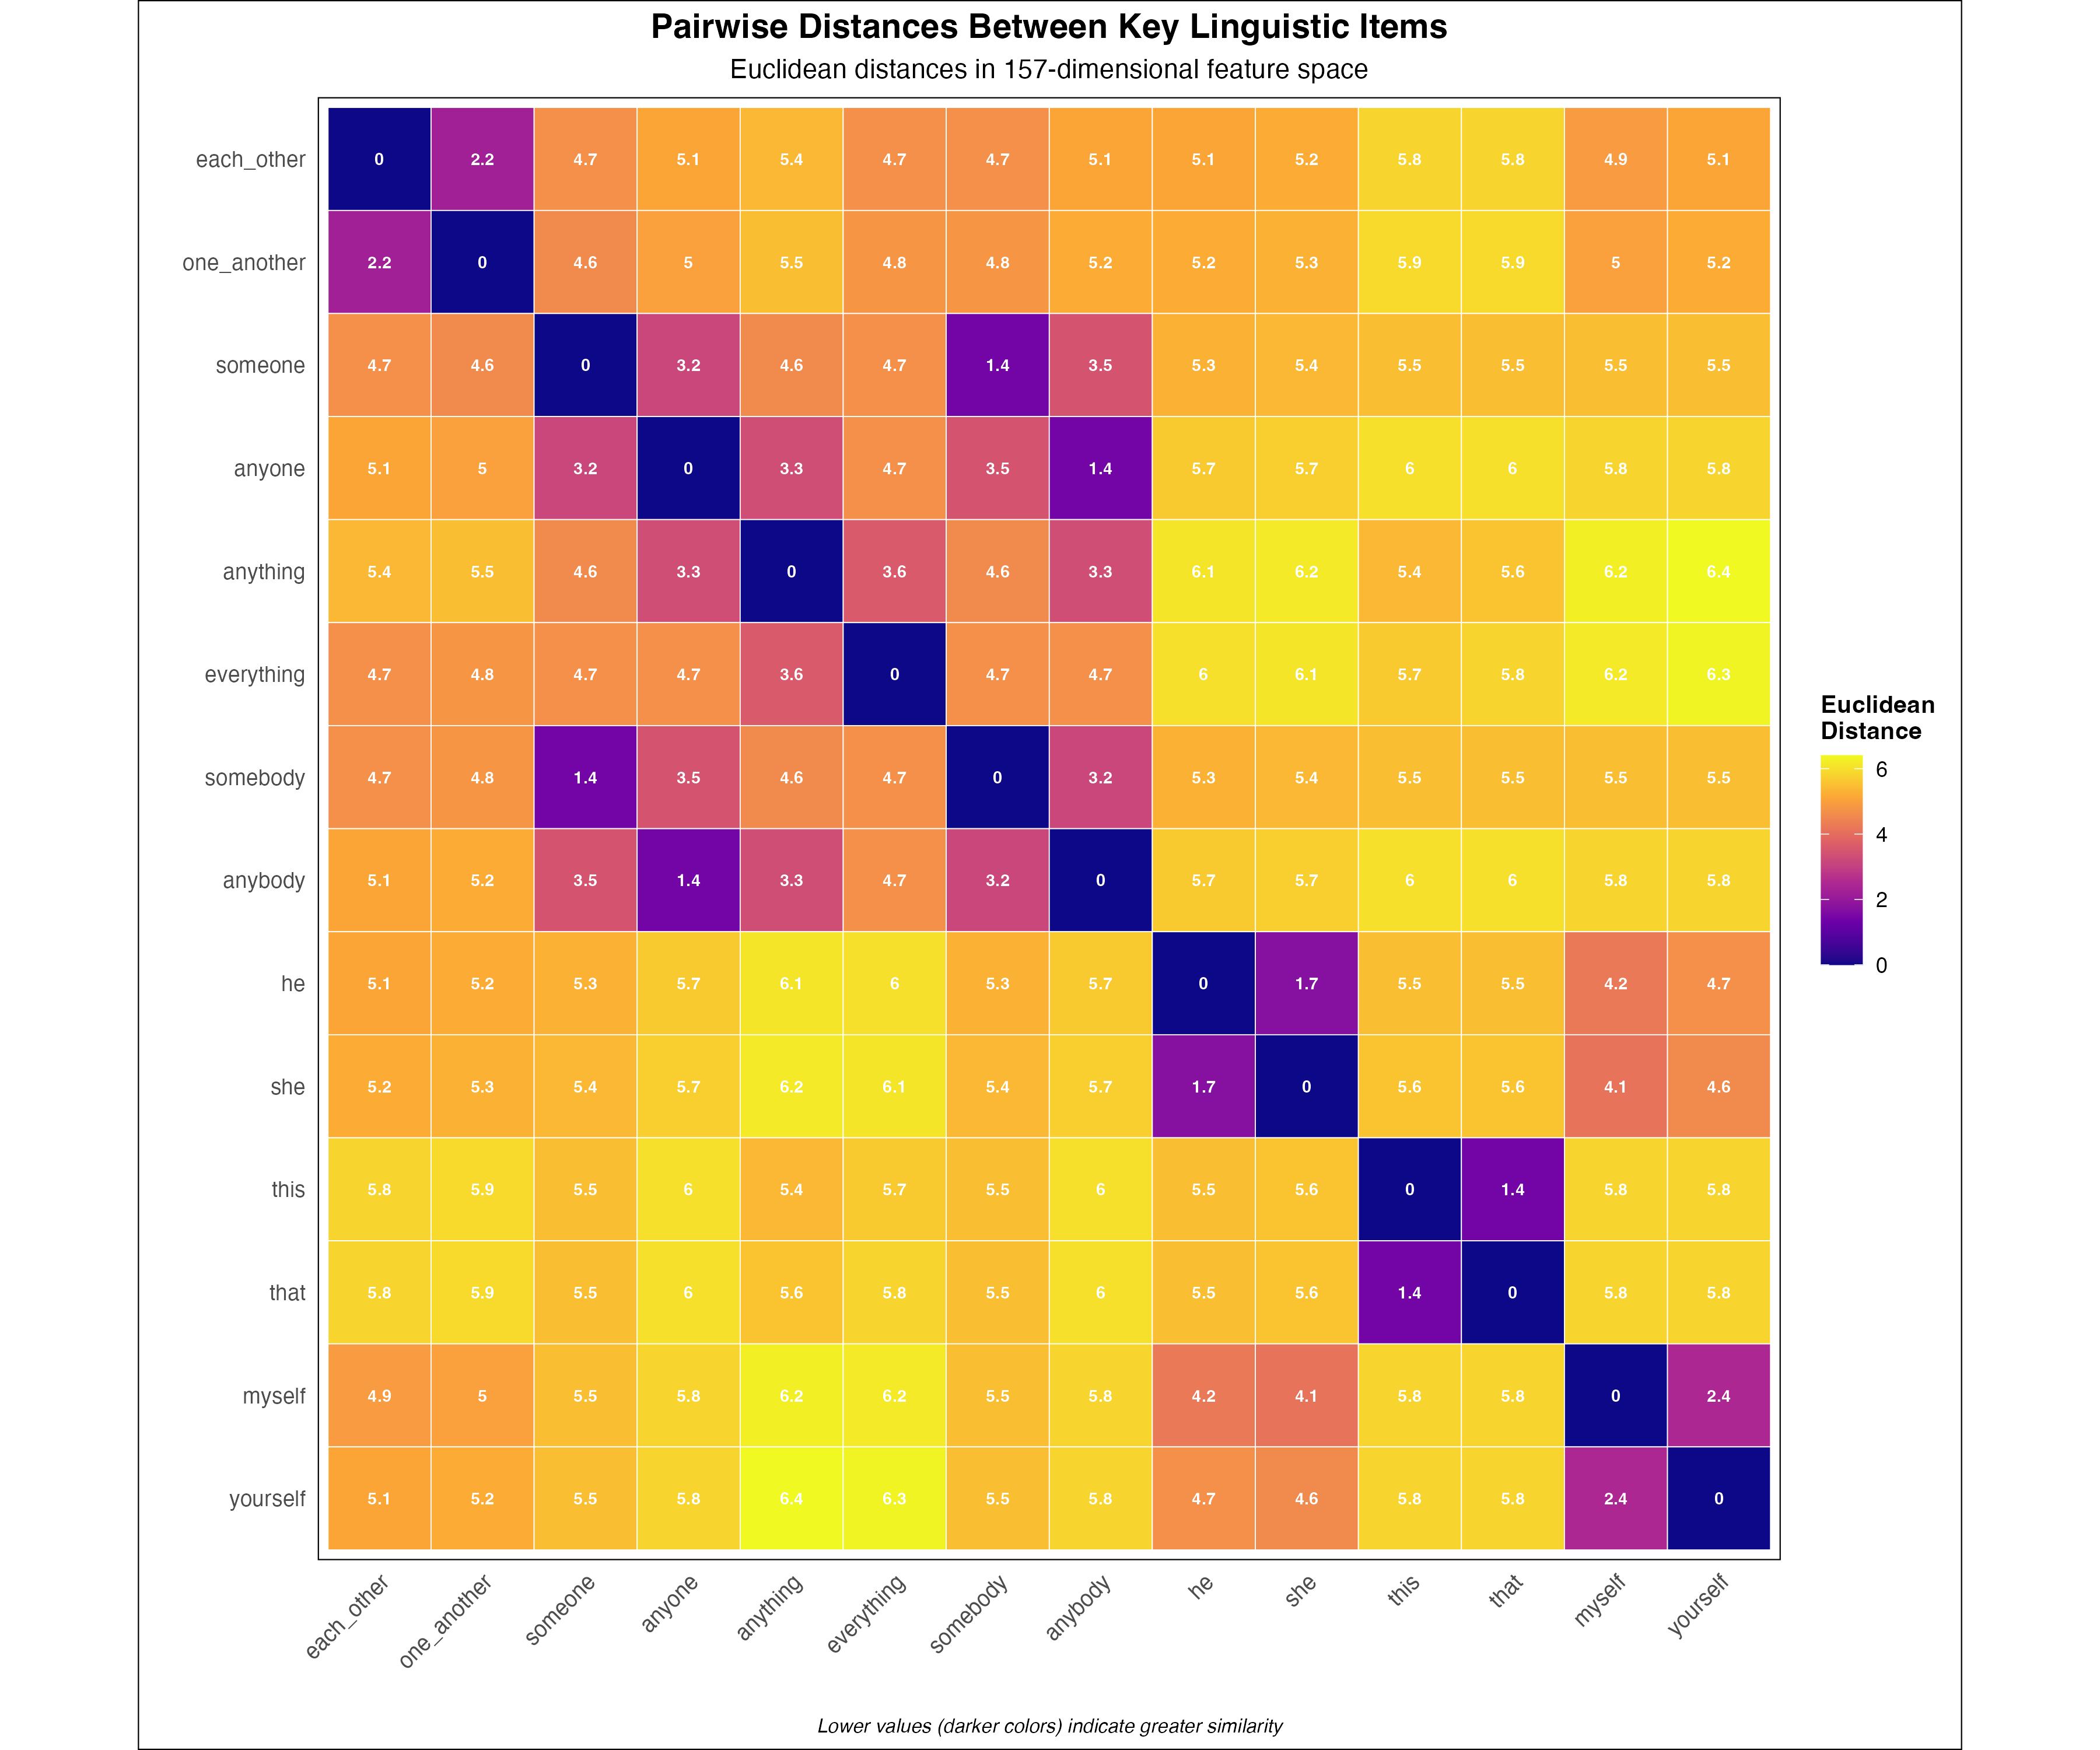
\includegraphics[width=0.9\textwidth]{reciprocals_distance_heatmap.png}
\caption{Distance heatmap showing pairwise Euclidean distances between key linguistic items. Reciprocals (\textit{each\_other}, \textit{one\_another}) show complex patterning, with somewhat closer average distances to fused determinatives (4.96) than to the selected pronouns (5.37) in this subset analysis.}
\label{fig:heatmap}
\end{figure}

The heatmap reveals interesting complexity in reciprocal patterning. While our comprehensive statistical tests favored pronoun classification, this focused distance analysis of key comparison items shows that reciprocals exhibit somewhat closer average distances to fused determinatives (4.96) than to the selected representative pronouns (5.37). This apparent contradiction highlights the importance of methodological choices in linguistic analysis and suggests that reciprocals may indeed occupy an intermediate grammatical position.

\subsection{Bayesian Analysis}

The Bayesian analysis incorporated strong prior probabilities (85\%) favoring the traditional pronoun classification based on scholarly consensus in major reference grammars. After observing the feature data, the posterior probability increased to 86.5\%, indicating that the empirical evidence provides additional support for the traditional classification.

The Bayes factor of 1.135 represents weak evidence favoring the pronoun classification. While not strong evidence, this factor combined with the robust prior knowledge results in high posterior confidence in the traditional analysis.

\subsection{Sensitivity Analysis}

Testing across different prior probability assumptions (ranging from 25\% to 95\% for pronoun classification) confirmed that our conclusions remain robust. Even with skeptical priors strongly favoring the determinative classification, the posterior probabilities consistently supported the traditional approach.

\section{Discussion}

\subsection{Convergent Evidence}

All four analytical methods—permutation testing, model comparison, ordination analysis, and Bayesian inference—converged on the same conclusion. This convergent evidence strengthens confidence in our findings and suggests that the results are not artifacts of any particular analytical approach.

The consistency across methods is particularly notable given their different theoretical foundations and statistical assumptions. Permutation tests make minimal distributional assumptions, model comparison focuses on predictive accuracy, ordination methods reveal global structure in high-dimensional data, and Bayesian analysis formally incorporates prior knowledge.

\subsection{Theoretical Implications}

Our findings have several implications for theories of grammatical classification:

\paragraph{Traditional Classification Vindicated}
The quantitative evidence strongly supports the traditional classification of reciprocals as pronouns found in major reference grammars. This suggests that established grammatical analyses often reflect genuine linguistic patterns detectable through comprehensive feature analysis.

\paragraph{Intermediate Grammatical Status}
Our analysis provides strong evidence that reciprocals occupy a genuinely intermediate grammatical position. While comprehensive statistical tests (permutation testing, model comparison, Bayesian analysis) favored pronoun classification, the focused distance analysis revealed closer similarity to fused determinatives. This methodological sensitivity, combined with relatively small effect sizes across analyses, confirms that reciprocals resist simple binary classification and exhibit properties of both categories depending on the analytical lens applied.

\paragraph{Fusion-of-Functions Framework}
The fusion-of-functions framework \citep{payne2007fusion} may still provide valuable theoretical insights even though our data do not support reclassifying reciprocals as fused determinatives. The framework's emphasis on gradient rather than discrete categories aligns with our finding of intermediate properties, suggesting that grammatical categories may be better understood as regions in multi-dimensional feature space rather than discrete classes.

\subsection{Methodological Considerations}

This study demonstrates both the value and the complexity of multi-method approaches in grammatical analysis. While different analytical techniques generally provided convergent evidence, the distance heatmap analysis revealed some divergent patterns, highlighting important methodological considerations.

The apparent contradiction between our comprehensive statistical tests (favoring pronoun classification) and the focused distance analysis (showing closer similarity to fused determinatives) illustrates how methodological choices can influence conclusions. This divergence likely reflects differences in:

\begin{itemize}
\item \textbf{Sample composition}: The heatmap used a smaller, curated set of representative items, while the comprehensive tests used all available pronouns
\item \textbf{Distance metrics}: Different approaches to measuring similarity in high-dimensional feature space
\item \textbf{Statistical weighting}: Whether all features contribute equally or are weighted by their discriminative power
\end{itemize}

This methodological sensitivity underscores the importance of transparency in analytical choices and suggests that reciprocals may indeed occupy a complex intermediate position that resists simple binary classification.

Our pre-registration approach helped avoid common pitfalls in exploratory data analysis. By establishing hypotheses and analytical plans before examining the data, we reduced the risk of finding spurious patterns or selectively reporting favorable results.

The incorporation of informative priors in Bayesian analysis represents a principled approach to integrating established linguistic knowledge with new empirical evidence. This framework can be particularly valuable in linguistic research where decades of scholarship provide substantial prior knowledge.

\subsection{Limitations}

Several significant limitations should be acknowledged:

\paragraph{Multiple Testing and Statistical Rigor}
Our analysis employed numerous statistical tests (permutation, model comparison, Bayesian inference, distance analysis) without correction for multiple comparisons, potentially inflating Type I error rates. Additionally, the high-dimensional nature of our data (157 features for 139 items) approaches regimes where distance-based methods become unreliable, which may explain some contradictory results between approaches.

\paragraph{Theoretical Assumptions}
Our methodology assumes that similarity in binary feature space corresponds to grammatical category membership. This strong assumption—that categories are determined by overall feature similarity rather than specific diagnostic properties—remains theoretically unjustified. Alternative models where categories depend on particular key features might yield different conclusions.

\paragraph{Feature Independence and Weighting}
We treated all 157 features as equally important and independent, though many are likely correlated. This violates assumptions of distance metrics and may create spurious clustering patterns. Some features may be far more diagnostic for category membership than others, but our equal-weighting approach cannot capture this.

\paragraph{Data Quality and Reliability}
The binary feature codings lack reported inter-annotator reliability statistics, and the encoding may lose important gradient information. Without understanding the reliability and validity of individual features, it becomes difficult to assess the robustness of patterns built upon them.

\paragraph{Methodological Sensitivity}
The apparent contradictions between our comprehensive statistical tests and focused distance analysis highlight problematic sensitivity to methodological choices. This suggests that conclusions about grammatical categories may depend critically on analytical decisions rather than reflecting stable linguistic properties.

\paragraph{Generalizability}
With only two reciprocal forms in English and a specific feature set, generalization is severely limited. Cross-linguistic investigation and alternative feature encodings are necessary to assess the broader validity of our findings.

\section{Conclusion}

This quantitative investigation reveals the complex grammatical status of English reciprocals \textit{each other} and \textit{one another}. While multiple analytical methods generally supported the traditional pronoun classification, our analysis also uncovered significant evidence for intermediate status that resists simple categorization.

The convergent evidence from permutation testing, model comparison, and Bayesian analysis favored pronoun classification, but focused distance analysis showed closer similarity to fused determinatives. This methodological sensitivity, combined with consistently small effect sizes, demonstrates that reciprocals occupy a genuinely intermediate position in grammatical space.

Rather than definitively supporting or rejecting the reclassification hypothesis, our findings highlight both the complexity of grammatical categorization and the challenges of quantitative approaches to linguistic classification. While reciprocals may indeed exhibit intermediate properties, the methodological sensitivity we observed—where different analytical approaches yield contradictory conclusions—suggests that some apparent complexity may reflect limitations in our analytical framework rather than purely linguistic phenomena.

Our methodological approach demonstrates the value of applying rigorous quantitative methods to theoretical linguistic questions. The combination of pre-registration, multiple analytical methods, and principled prior incorporation provides a framework for testing grammatical hypotheses that could be productively applied to other classification questions in linguistics.

Future research might profitably examine reciprocal systems cross-linguistically, investigate additional feature dimensions, or apply similar quantitative approaches to other contested grammatical classifications. The apparent methodological sensitivity observed here also suggests the value of explicitly testing how analytical choices affect conclusions in grammatical classification studies. The methods developed here provide a template for empirically grounded approaches to theoretical linguistic questions while highlighting the importance of methodological transparency and multiple analytical perspectives.

\section*{Acknowledgments}

We thank [relevant parties] for discussions that improved this work. All remaining errors are our own.

\bibliographystyle{plainnat}
\begin{thebibliography}{9}

\bibitem{gelman2013bayesian}
Gelman, A., Carlin, J. B., Stern, H. S., Dunson, D. B., Vehtari, A., \& Rubin, D. B. (2013). 
\textit{Bayesian data analysis}. CRC press.

\bibitem{huddleston2002cambridge}
Huddleston, R., \& Pullum, G. K. (2002). 
\textit{The Cambridge grammar of the English language}. 
Cambridge University Press.

\bibitem{payne2007fusion}
Payne, J., Huddleston, R., \& Pullum, G. K. (2007). 
Fusion of functions and the structure of the determiner phrase. 
In \textit{Language and Linguistics}, 8(2), 295-318.

\end{thebibliography}

\end{document}